\chapter{State of the Art}
\label{cha:2nd_chapter}
In this chapter we first present the related work on the Generative Adversarial Networks in the literature (\ref{sec:related_work}) and then, in Section \ref{sec:theoretical_background}, we introduce the theoretical aspects our work is based upon, while giving the reader an overview of the tools and techniques we applied in our models, in order to better understand the setting in which our work takes place.

\section{Related Work}
\label{sec:related_work}
\ac{GAN}s have been used in many data domains, but the images one is where this type of neural network obtained the most significant results so far. In \cite{gan} this architecture has been tested for the first time on a range of image datasets including MNIST\cite{lecun}, the Toronto Face Database\cite{tfd} and CIFAR-10\cite{cifar}. Isola et al. applied \ac{GAN}s to the image-to-image translation task and, in order to explore the generality of their work\cite{pix2pix}, experimented with a variety of settings and datasets such as generating the night version of an image whose daily version was given as input to the network or synthesizing the picture of a building by only observing its relative architecture label as input after a training performed on CMP Facades 
(Figure~\ref{fig:first_figure}).
\begin{figure}[htbp!]
\centering
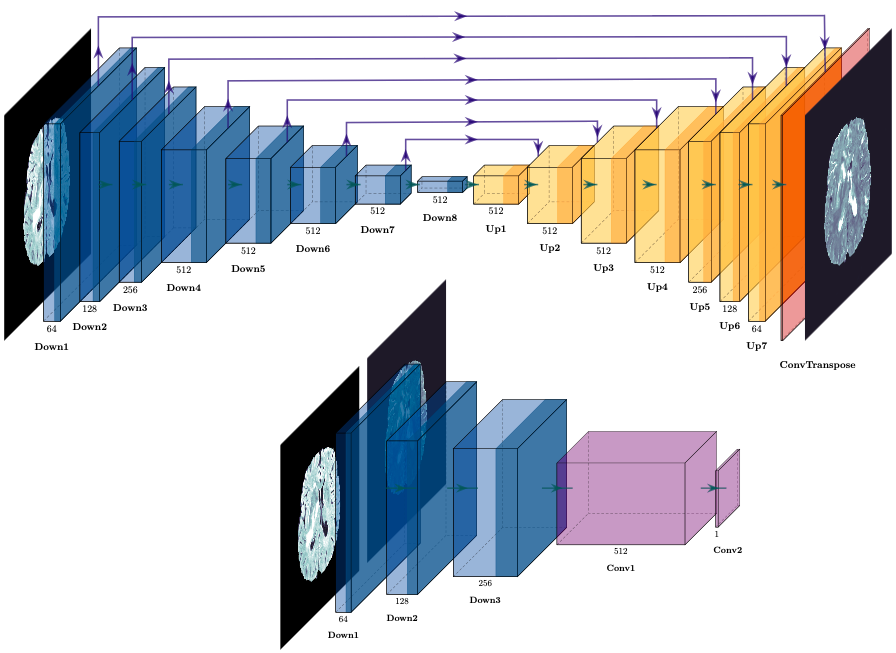
\includegraphics[height=0.235\textheight]{images/pix2pix}
\caption[Pix2Pix example from Isola et al.]{Examples of image-to-image translation from the work of Isola et al. \cite{pix2pix}}
\label{fig:first_figure}
\end{figure}
\subsection{GANs in Medical Imaging}
\label{subsec:gans_medical_imaging}
Countless studies about medical image synthesis were approached using \ac{GAN}s. In particular, cross modality image synthesis (so the conversion of the input image of one modality to the output of another modality) is the most important application of this architecture: in 2018, was even published a review\cite{Yi_2019} about all the work and progresses that have been done in the field of medical imaging through the application of~\ac{GAN}s. The authors described the magnetic resonance as the most common imaging modality explored in the literature related to this generative approach invented by Goodfellow and this is probably due to the fact that~\ac{GAN}s, through the cross modality synthesis, can reduce the excessive amount of time requested from~\ac{MR} acquisition.

\vspace{5mm} %5mm vertical space
Many different approaches and datasets have been used in the literature in order to overcome the problem of missing modalities. Orbes-Arteaga et al., in \cite{flair&t1}, since most of the datasets contain only $T_1$ or $T_1$/$T_2$/PD scans due to logistical reasons, implemented a~\ac{GAN} that generates $T_{2flair}$ of the brain using $T_1$ modality. 
In \cite{lapgan}, Camileri et al. developed a variant of the original GAN, called Laplacian pyramid framework (LAPGAN) that synthesizes images in a coarse-to-fine way. This method, as the name suggests, is based on Laplacian pyramid and allows to generate initially an image with low resolution and then, incrementally, add details to it. Another approach to generate missing modalities was proposed in \cite{double_scenario} where they presented two possible scenarios, based on the given dataset: they use a model called pGAN (that incorporates a pixel-wise loss into the objective function) when the multi-contrast images are spatially registered while they adopt a cycleGAN\cite{cycle_gan}  in the more realistic scenario in which pixels are not aligned between contrasts. A cycleGAN is a~\ac{GAN} variant characterized by the fact that has two generators, two discriminators and uses a cycle consistency loss with a collection of training images from the source and target domain that don't need to be related in any way.

Most of the papers about Generative Adversarial Networks, and also this work, though, are based on a training performed using paired examples, with input image and target image perfectly aligned. 

\vspace{5mm} %5mm vertical space
It is worth to cite also the work done by Anmol Sharma and Ghassan Hamarneh that were, to the best of their knowledge\cite{migan}, the first to propose a many to many generative model, capable of synthesize multiple missing sequences given a combination of various input sequences. Furthermore, they were the first to apply the concept of curriculum learning, based on the variation of the difficulty of the examples that are shown during the network training.

\vspace{5mm} %5mm vertical space
MRI isn't the only imaging technique where~\ac{GAN} has been applied to: in literature is possible to find various publications of generative models that use~\ac{PET},~\ac{CT} or~\ac{MRA} images. 
Olut et al., in 2018, demonstrated that~\ac{GAN} works efficiently even when the source imaging technique is different from the target one: they were the first ones to synthesize~\ac{MRA} brain images from $T_1$ and $T_2$ MRI modalities\cite{mra&mri}. Ben-Cohen et al. published in the same year an article\cite{ct&pet} explaining how to generate~\ac{PET} images using~\ac{CT} scans through a fully connected neural network, whose output is improved and refined by a~\ac{cGAN}\cite{cgan}.


\vspace{5mm} %5mm vertical space
The work related to the generation of medical image is huge and new papers about the topic are being published every week. Many approaches have been already tested and many datasets have been used but there are still lots of challenges that need to be solved in order to be able to be employed in medical imaging\cite{Yi_2019} and since there is still room for improvements in the application of generative models in medical imaging, we present in this work a complete study on different architectures of~\ac{GAN} used to generate missing modalities of brain scans, followed by an analysis of the information that passes through the inner channels and through the skip connections of the generator networks.


\section{Theoretical Background}
\label{sec:theoretical_background}
The architecture of the main model used in our work, the Generative Adversarial Network, is based on the Convolutional Neural Network: a deep neural network with many hidden layers that nowadays is proved successful in many application going from Image Recognition to Video Analysis, passing through Natural Language Processing, Anomaly detection, Drug Discovery, etc.

\subsection{Convolutional Neural Network}
\label{sec:convolutional_neural_network}
The 1980, period in which David H. Hubel and Torsten Wiesel gave crucial insights about the structure of the visual cortex (the researchers are winners of the 1981 Nobel Price in Physiology or Medicine for their work), is the starting point from which \textit{convolutional neural networks} started to gradually evolve into what is today the architecture most used in~\ac{DL}.

\vspace{5mm} %5mm vertical space
The milestone is represented by the work of Yann LeCun that in 1998 developed a model, LeNet-5, to identify handwritten digits for zip code recognition in the postal service\cite{lecun}.
This model was composed by traditional building blocks such as fully connected layers and sigmoid activation functions but also by convolutional layers and pooling layers, introduced for the first time.

The most important building block is the convolutional layer, based on the mathematical operation from which~\ac{CNN} take its name. This layer allows to extract features by convolving the input with a certain number of filters, producing a stack of feature maps, one per each filter that was convolved with the input image.
Each filter basically tries to capture, in the first layers of the network, low-details of the image by producing this feature map that highlights which are the areas on the input that were activated by the filter the most.
In the the next hidden layers this small low-level features are assembled into higher-level features and this hierarchical structure is one of the reason why~\ac{CNN}s work so well and are so widely used\cite{lecun}.

\subsection{Generative Adversarial Network}
\label{subsec:gan}
Generative Adversarial Network was proposed in 2014 by Ian J. GoodFellow\cite{gan} and represents a new framework for estimating generative models in an adversarial setting. The system is composed by two neural networks: a discriminator D, typically a~\ac{CNN}, and a generator G that are trained simultaneously. 

\begin{figure}[H]
\centering
\includegraphics[height=0.27\textheight]{images/GANs.pdf}
\caption[Generative Adversarial Network Framework]{Generative Adversarial Network Framework \cite{GAN_image}.}
\label{fig:GANs}
\end{figure}
In particular, G is trained to learn the probability distribution of the data given as input and to generate synthesized data that exhibits similar characteristics to the authentic data while the discriminative model estimates the probability that a sample came from the training data rather than G.

\vspace{5mm} %5mm vertical space
This adversarial setting is usually explained through the example of the counterfeiter (generator) that tries to produce and use fake money without being caught from the police (discriminator) that, on the other hand, tries to detect the counterfeiter fake currency. The process continues until the counterfeiter becomes able to trick the police with success. \ac{GAN}s work in the same way, with the two networks that compete with each other in a game (corresponding to what is called minimax two-player game in Game Theory \cite[p.~276]{optimization}): the discriminator tries to distinguish true images, belonging to the input dataset, from fake images produced by the generator, whose objective is instead to learn to generate the most realistic data possible to be able to fool D.

Equation~\ref{eq:first_equation} shows the losses for D and G used in the original architecture\cite{gan}.

\begin{equation} \label{eq:first_equation}
\begin{gathered}
L_D^i \leftarrow \frac{1}{m} \sum_{i=1}^{m} [\log D(x^{(i)}) + \log(1 - D(G(z^{(i)})))] \\
L_G^i \leftarrow \frac{1}{m} \sum_{i=1}^{m} \log(1 - D(G(z^{(i)})))
\end{gathered}
\end{equation}
where $z^i$ is a batch of random noise and $x^i$ is a batch of true \textit{m} data samples.
The two networks are trained alternately using \textit{Backpropagation}, in such a way that the generator can learn to synthesize the images based on the discriminator feedback. 

It's important to highlight that the G never sees real images: it just learns the gradients flowing back through the discriminator. The better the discriminator gets, the more information about real images is contained in these secondhand gradients, so the generator can make significant progress\cite[p.~1301]{hands_on_ml}.
As the training advances, the~\ac{GAN} may end up in a situation that is called \textit{Nash equilibrium}, so a situation in which the generator produces perfectly realistic images while the discriminator is forced to guess (50\% real and 50\% fake). Unfortunately, even training a GAN for a long time, there is no guarantee to reach this equilibrium\cite[p.~1307]{hands_on_ml}. 

\subsection{Deep Convolutional GAN (DCGAN)}
\label{subsec:dcgan}
The problem with the original~\ac{GAN} paper \cite{gan} is that GoodFellow et al. experimented with convolutional layers but only with small images.
In the following months researchers tried to work with deeper neural networks for larger images and, in 2015, Radfrod, Metz and Chintala presented an improved version of the original architecture with some tricks and variations\cite{dcgan}.


The guidelines proposed, that we followed in our work, in order to obtain a stable training even with large images, are: 
\begin{itemize}
  \item Replacement of any pooling layers (downsampling layers that allow to reduce the spatial information of the image) with strided convolutions in the discriminator and with transposed convolutions (similar to the convolution layer but goes in the opposite direction by enlarging the spatial dimensions) in the generator.
  \item Batch normalization\cite{batchnormalization} - a normalization of the input computed across the whole batch - in every layer (with the exception of the generator output layer and the discriminator input layer).
  \item Remove fully connected hidden layers (whose neurons are connected to every node of the previous layer), both in G and D.
  \item ReLu as activation functions\cite{relu} in G for all layers except for the output, which uses tanh (hyperbolic tangent activation function with an output range from -1 to +1). ReLu is a non linear function that maps its input between 0 to infinity.
  \item use of Leaky ReLU: activation function similar to ReLU but with a small slope for negative values that avoid neurons to stop outputting anything other than a 0 value. It is used in D for all layers.
\end{itemize}

\begin{figure}[htbp!]
\centering
\includegraphics[height=0.25\textheight]{images/dcgan}
\caption[Layers from DCGAN, Radford, Metz, and Chintala]{DCGAN generator used in the work of Radford, Metz and Chintala.}
\label{fig:dcgan}
\end{figure}

\subsection{Conditional GAN}
\label{subsec:conditional_gan}
In the \textit{Conclusions and future work} of the original~\ac{GAN} paper\cite{cgan}, GoodFellow et al. suggested that the proposed framework could have been extended by conditioning the input of both G and D.
This extension was realized by Mehdi Mirza and Simon Osindero that developed a Conditional Generative Adversarial Net.
The authors explain that in a unconditioned generative setting there is no possibility to control the modes of the data that is generated, while, by conditioning the input with some extra information \textit{y}, it's possible to direct the data generation process\cite{cgan}.

Such extra input can be any kind of auxiliary information, such as class labels or data coming from other modalities (in our work we conditioned the input with images as extra information), so the prior noise \textit{z} is combined to \textit{y} as input to the generator while the discriminator takes as input data \textit{x} and \textit{y.}


\subsection{Image-to-Image translation with Conditional GAN}
\label{subsec:image-to-image_translation}
After the publication, in 2015, of \textit{Conditional Adversarial Nets}\cite{cgan}, many researchers started to apply this kind of architecture to the \textit{Image-to-Image translation}, the task of translating one possible representation of a scene into another one,  using images as auxiliary information to control the data generation. An important contribute was given by Phillip Isola et al. that developed a general framework that is not application-specific and is generally known as Pix2Pix\cite{pix2pix}.

\vspace{5mm} %5mm vertical space
Pix2Pix works so well in many domains because of several architectural choices that were adopted both in the generator and in the discriminator.

\begin{figure}[htbp!]
\centering
\includegraphics[height=0.165\textheight]{images/pix2pix_2}
\caption[Samples from Pix2Pix, Isola et al.]{Thermal images translated to RGB photos: an example of Image-to-Image translation using Pix2Pix\cite{pix2pix}.}
\label{fig:pix2pix_2}
\end{figure}


None of these architectural choices were introduced for the first time by the authors of Pix2Pix: they have been already explored in many papers related to~\ac{GAN} and focused on specific applications, but for the first time they have been used for a general-purpose solution to image-to-image translation.
The neural networks chosen by Isola et al. are the same ones that have been used in our work: a "U-Net"-based architecture\cite{unet} as generator and a "PatchGAN" classifier, similar to the one proposed in\cite{patchgan}, as discriminator. 

Furthermore, the authors found beneficial to mix the~\ac{GAN} objective to a more traditional loss such as the L1 loss.
So, in addition to the objective of a conditional GAN, that can be expressed as
%\Bigg
\begin{equation} \label{eq:objective_gan}
\mathcal{L}_{cGAN}(G,D) = \mathbb{E}_{x,y} [\log D(x, y)] + \mathbb{E}_{x,z} [\log (1 - D(x, G(x, z)))], 
\end{equation}

where G tries to maximize the objective against the adversarial D that tries to minimize it, a L1 loss was used in order to measure the distance between the ground truth image and the generated image:

\begin{equation} \label{eq:l1_loss}
\mathcal{L}_{L1}(G) = \mathbb{E}_{x,y,z} [\| y - G(x,z) \|_1].
\end{equation}

L1 loss is preferred to the L2 one, since it produces results less blurred. 
The final objective, then, is:

\begin{equation} \label{eq:final_objective}
G^* = \arg\min_{G}\max_{D} \mathcal{L}_{cGAN}(G,D) + \lambda \mathcal{L}_{L1}(G).
\end{equation}

Pix2pix is the model whose performances are used as baseline in our work and, because of this, we present below further details on the U-Net architecture and on the PatchGAN architecture, in order to make more understable the next chapters.

\vspace{6mm} %5mm vertical space
\noindent\textbf{U-Net}

\vspace{2mm} %5mm vertical space
\noindent Pix2pix adopts as generator a U-Net architecture\cite{unet}, that allows to obtain better results with respect to the ones reached by generators composed by an encoder-decoder network (Figure \ref{fig:unet2}).


The important problem in image-to-image translation, so in a setting where we need to map a high resolution input grid to a high resolution output grid, by maintaining the same underlying structure between an input and output image that differ in surface appearance\cite{pix2pix}, is that, using an encoder-decoder network, the input image is simply downsampled progressively until a bottleneck layer, after which the process is reversed and the information passes through many upsample layers.

Because of this bottleneck layer, it would be preferable to have to shuttle all this information directly across the net: this is obtained adding to the network some links, called \textbf{skip connections} between, for example, the \textit{i} layer and the \textit{n-i} layer, where \textit{n} is the total number of layers. 

\vspace{6mm} %5mm vertical space
Skip connections result very useful in tasks such as image colorization, where input and output share the location of the prominent pixels, and are able to prevent the problem of losing information through the bottleneck.

\begin{figure}[H]
\centering
\includegraphics[height=0.18\textheight]{images/unet2.pdf}
\caption[Generator architectures in Pix2Pix network]{Two choices for the generator architecture. U-Net has skip connections between mirrored layers\cite{pix2pix}.}
\label{fig:unet2}
\end{figure}


%\vspace{6mm} %5mm vertical space
\noindent\textbf{PatchGAN}

\vspace{2mm} %5mm vertical space
\noindent Isola et al. explain that, since L1 loss (Eqn.~\ref{eq:l1_loss}) is able to capture accurately low-level frequencies, it's sufficient to restrict the~\ac{GAN} discriminator focus only on the high frequencies.
High frequencies can be captured by using a~\ac{CNN}, called \textit{Patch}GAN\cite{patchgan}, that is able to discriminate small local \textit{NxN} patches of the images and assign to these a fake or true label. Averaging all the responses across the image provides then the ultimate output of D\cite{pix2pix}.

The authors demonstrate, after testing various kinds of patches, such as a 1x1 "PixelGAN" and a 286x286 "ImageGAN", that a 70x70 PatchGAN gives the best results in terms of blurriness, sharpness, general quality of the image and presence of any artifacts (Fig.\ref{fig:nxn})

\begin{figure}[H]
\centering
\includegraphics[height=0.079\textheight]{images/nxn.pdf}
\caption[Patch size variations in PatchGAN discriminator]{Path size variations going from 1x1 "PixelGAN" to "286x286" "ImageGAN" passing through the 70x70 PatchGAN that produces sharp results in both the spatial and spectral (colorfulness) dimensions\cite{pix2pix}.}
\label{fig:nxn}
\end{figure}

Furthermore, scaling the patch beyond 70x70 doesn't improve the quality of the output and has the downside of a longer training needed, because of the larger number of parameters.

\section{Summary}
\label{sec:2nd_section_summary}
In this chapter we presented the solution proposed in the last years, thanks to recent improvements in \ac{DL}, to the problem of missing modalities.

After this, we described the main architectures upon which is based our work, starting from the original~\ac{GAN} and going through all the theory behind generative adversarial networks, giving to the reader a solid background about Deep Convolutional~\ac{GAN}, Conditional~\ac{GAN} and the two networks that compose Pix2Pix: U-Net as generator and PatchGAN as discriminator. Theory that is needed in order to understand the next chapters and in particular chapter 4 that shows how we implemented the network architecture in our system.